\documentclass[tikz,border=2pt]{standalone}
\usepackage{amsmath,amssymb}
\usepackage{tikz}
\usetikzlibrary{arrows.meta,matrix}

\begin{document}
% A pivot is the first nonzero entry of a row; its column is a pivot column (a basic variable),
% the other columns carry free variables.
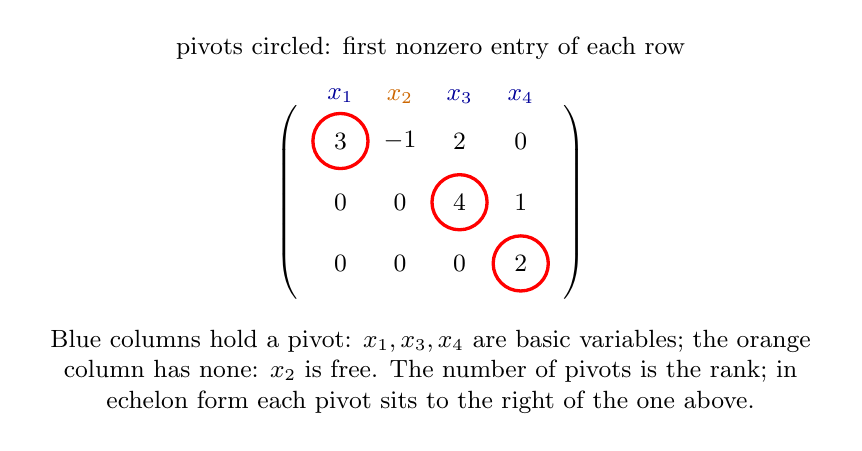
\begin{tikzpicture}[every node/.style={font=\small}, >={Latex[length=1.6mm]}]
	\matrix (A) [matrix of math nodes, nodes={minimum size=7mm, anchor=center}, left delimiter=(, right delimiter=), column sep=1pt, row sep=1pt] at (0,0) {
		|[draw=red, very thick, circle, inner sep=1pt]| 3 & -1 & 2 & 0 \\
		0 & 0 & |[draw=red, very thick, circle, inner sep=1pt]| 4 & 1 \\
		0 & 0 & 0 & |[draw=red, very thick, circle, inner sep=1pt]| 2 \\
	};
	\node[anchor=south, yshift=12pt] at (A.north) {pivots circled: first nonzero entry of each row};
	\foreach \c in {1,3,4} {\node[blue!60!black, anchor=south] at (A-1-\c.north) {$x_{\c}$};}
	\node[orange!80!black, anchor=south] at (A-1-2.north) {$x_2$};
	\node[anchor=north, align=flush center, text width=10cm] at (0,-1.5) {Blue columns hold a pivot: $x_1,x_3,x_4$ are basic variables; the orange column has none: $x_2$ is free. The number of pivots is the rank; in echelon form each pivot sits to the right of the one above.};
\end{tikzpicture}
\end{document}
